\documentclass[twoside]{../zirkelblatt1415}
\usepackage{mathtools}
\usepackage{wrapfig}
\usepackage{tabto}
\usepackage{booktabs}
\usepackage{relsize}
\let\raggedsection\centering

\theoremstyle{definition}
\newtheorem{defn}{Definition}[section]
\newtheorem{defn'}{Vorläufge Definition}[section]
\newtheorem{axiom}[defn]{Axiom}
\newtheorem{bsp}[defn]{Beispiel}

\theoremstyle{plain}

\newtheorem{prop}[defn]{Proposition}
\newtheorem{motto}[defn]{Motto}
\newtheorem{wunder}[defn]{Wunder}
\newtheorem{ueberlegung}[defn]{Überlegung}
\newtheorem{lemma}[defn]{Lemma}
\newtheorem{kor}[defn]{Korollar}
\newtheorem{hilfsaussage}[defn]{Hilfsaussage}
\newtheorem{satz}[defn]{Satz}
\newtheorem{thm}[defn]{Theorem}

\theoremstyle{remark}
\newtheorem{bem}[defn]{Bemerkung}
\newtheorem{warnung}[defn]{Warnung}
\newtheorem{aufg}[defn]{Aufgabe}

\definecolor{darkred}{rgb}{0.7,0,0}
\definecolor{shadecolor}{rgb}{.95,.95,.95}

\newenvironment{listing}{
  \renewcommand*\theenumi{\arabic{enumi}}
  \renewcommand{\labelenumi}{\theenumi.}
  \begin{enumerate}\itemsep0em}{\end{enumerate}}

\newcommand{\defeq}{\vcentcolon=}
\newcommand{\prim}[1]{\text{\textnormal{$#1$ prim}}}
\newcommand{\bigsum}{\mathop{\mathlarger{\mathlarger{\sum}}}}
\newcommand{\bigprod}{\mathop{\mathlarger{\mathlarger{\prod}}}}

\DeclareMathOperator{\ld}{ld}

\usepackage{mathpazo}

\begin{document}

\maketitleCustom{Klassen 10/11/12}{\textbf{\textsf{%
  Analytische Zahlentheorie \\
  \normalsize Zirkelzettel vom 5. und 19. Dezember 2014}}}

\begin{center}
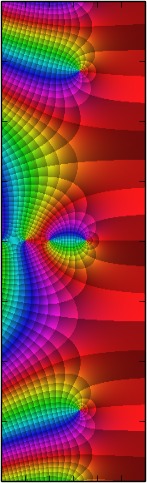
\includegraphics[angle=90]{zeta-function-complex}

\vspace{0.4cm}
\begin{minipage}{0.9\textwidth}
\scriptsize Die Werte der Riemannschen~$\zeta$-Funktion auf einem Streifen um den
Ursprung in der komplexen Zahlen\-ebene (um 90~Grad gedreht).
\url{http://en.wikipedia.org/wiki/File:Riemann-Zeta-Detail.png}\par
\end{minipage}
\end{center}

\vspace{1em}
{\renewcommand{\addvspace}[1]{\vskip0.6em}
\tableofcontents%
}

\newpage

\section{Der Fundamentalsatz der Arithmetik}

\begin{defn}Eine \emph{Primzahl} ist eine positive natürliche Zahl, die
\emph{genau zwei} verschiedene positive Teiler besitzt.\end{defn}

Gemäß dieser Definition beginnt die Folge der Primzahlen also mit
\[ 2, \quad 3, \quad 5, \quad 7, \quad 11, \quad 13, \quad 17, \quad \ldots \]
Die Zahl~$1$ zählt nicht als Primzahl -- sie besitzt als einzigen Teiler sich
selbst und hat daher nicht zwei verschiedene Teiler.

\begin{thm}[Fundamentalsatz der Arithmetik]Jede positive natürliche Zahl lässt
sich auf eindeutige Art und Weise als Produkt von Primzahlen
schreiben.\end{thm}

\begin{proof}Sei eine beliebige natürliche Zahl~$n$ gegeben. Falls~$n$ eine
Primzahl ist, haben wir damit die gesuchte Zerlegung in Primfaktoren schon
gefunden. Falls~$n$ keine Primzahl ist, spaltet sich~$n$ in ein Produkt auf: $n
= a \cdot b$, und wir können mit der Suche nach einer Zerlegung bei~$a$ und~$b$
fortfahren.

Die Eindeutigkeitsaussage ist interessanter (Aufgabe~\ref{aufg:eindt}).\end{proof}

\begin{aufgabe}{Primfaktorzerlegung der Eins}
Der Fundamentalsatz der Arithmetik behauptet, dass sich \emph{jede} positive
natürliche Zahl in Primfaktoren zerlegen lässt. Die Zahl~$1$ ist auch eine
solche positive natürliche Zahl. Siehst du, wie sich diese zerlegen lässt?

\emph{Hinweis.} Das ist etwas versteckt. Beachte, dass~$1$ keine Primzahl ist.
\end{aufgabe}

\begin{aufgabe}{Soll Eins eine Primzahl sein?}
Es gibt ein gutes mathematisches Argument, wieso es sinnvoll ist, die Eins
nicht als Primzahl zu definieren. Finde es!

\emph{Tipp.} Denke an die Eindeutigkeit der Primfaktorzerlegung. Was wäre, wenn
man die Zahl Eins als Primzahl zulassen würde?
\end{aufgabe}

\begin{aufgabe}{Eindeutigkeit der Primfaktorzerlegung}\label{aufg:eindt}
Mit dieser Aufgabe beweisen wir, dass die Zerlegung einer Zahl in Primfaktoren
bis auf Umordnung der Faktoren eindeutig ist. In Formeln ausgedrückt: Gilt
\[ p_1 \cdots p_n = q_1 \cdots q_m, \]
wobei~$p_1,\ldots,p_n$ und~$q_1,\ldots,q_m$ Primzahlen sind, so folgt schon~$n
= m$ (links und rechts stehen also gleich viele Faktoren) und jeder Faktor der
linken Seite tritt auch genau einmal auf der rechten Seite auf und umgekehrt.

\begin{enumerate}
\item Zeige zuerst: Teilt eine Primzahl~$p$ ein Produkt~$a \cdot b$, so
teilt~$p$ schon~$a$ oder~$p$ teilt~$b$. In Formeln:
\[ \text{Wenn $p \mid ab$, dann $p \mid a$ oder $p \mid b$.} \]

\emph{Tipp.} Das ist gar nicht so leicht. Verwende, dass die Zahlen~$a$ und~$p$
irgendeinen größten gemeinsamen Teiler~$d$ haben, und dass sich dieser in der
Form~$d = fa + gp$ für gewisse Zahlen~$f$ und~$g$ schreiben lässt. (Eine solche
Darstellung des größten gemeinsamen Teilers heißt \emph{Bézoutdarstellung}.
Dass es eine solche immer gibt, folgt aus dem \emph{euklidischen Algorithmus}.)

\item Beweise mit dem Resultat aus Teilaufgabe~a) die Eindeutigkeitsbehauptung.
\end{enumerate}\fixlistspacing
\end{aufgabe}

\begin{aufgabe}{Primzahlen mögen Vielfache der Sechs}
Beweise: Jede Primzahl größer als~$3$ liegt benachbart zu einem Vielfachen
von~$6$. In Formeln: Ist~$p > 3$ eine Primzahl, so teilt~$6$ entweder~$p-1$
oder~$p+1$.

\emph{Tipp.} Eine Zahl ist genau dann ein Vielfaches von~$6$, wenn sie ein
Vielfaches von~$2$ und von~$3$ ist. Weißt du von den drei Zahlen~$p-1$,~$p$
und~$p+1$, ob sie ein Vielfaches von~$3$ sind?
\end{aufgabe}


\section{Die Entdeckung der Irrationalität}

\begin{defn}Eine reelle Zahl~$x$ heißt genau dann \emph{rational}, wenn sie
sich als Quotient zweier ganzer Zahlen schreiben lässt: $x = a/b$ für gewisse
ganze Zahlen~$a$ und~$b$.\end{defn}

Dass nicht alle Zahlen rational sind, war eine erstaunliche Entdeckung im
fünften Jahrhundert~v.~Chr. Manche sehen diese Erkenntnis sogar als
Geburtsstunde der modernen Mathematik an. Als Entdecker der
Irrationalität gilt der griechische Mathematiker Hippasos von Metapont. Er
erkannte, dass der \emph{goldene Schnitt} irrational ist. Damit erschütterte er
die Schule der Pythagoreer, denn diese waren von dem Kredo \emph{Alles ist
Zahl} überzeugt, wobei sie mit "`Zahl"' \emph{rationale Zahl} meinten.
Ironischerweise kam der goldene Schnitt auch noch im Erkennungszeichen der
Pythagoreer vor, dem Pentagramm.

\begin{thm}Die Zahl~$\sqrt{2}$ ist nicht rational.\end{thm}

\begin{aufgabe}{Irrationalität von Quadratwurzeln}
\begin{enumerate}
\item Beweise, dass~$\sqrt{2}$ nicht rational ist.

\emph{Tipp.} Gehe nach folgendem Muster vor. Angenommen,~$\sqrt{2}$ ist doch
rational. Nach Definition gibt es dann ganze Zahlen~$a$ und~$b$ mit~$\sqrt{2} =
a/b$. Quadrieren und Umstellen zeigt~$2 b^2 = a^2$. Überlege nun, wie oft der
Primfaktor~$2$ auf den beiden Seiten dieser Gleichung vorkommt.

\item Beweise, dass für jede Primzahl~$p$ die Zahl~$\sqrt{p}$ nicht rational
ist.

\item Beweise, dass für jede Zahl~$n$, in deren Primfaktorzerlegung mindestens
eine Primzahl ungerade oft vorkommt, die Zahl~$\sqrt{n}$ nicht rational ist.
\end{enumerate}\fixlistspacing
\end{aufgabe}

\begin{aufgabe}{Anschauliche Bedeutung von Quadratwurzeln}
Wenn Quadratwurzeln sehr seltsame Zahlen ohne praktische Bedeutung wären,
hätte die Entdeckung der Irrationalität vielleicht einen geringeren
Stellenwert. Tatsächlich aber kommen Quadratwurzeln in der
Geometrie überall vor: Finde eine geometrische Figur, deren Kantenlängen alle
ganze Zahlen sind, sodass eine weitere eingezeichnete Hilfslinie aber
irrationale Länge hat.
\end{aufgabe}

\begin{aufgabe}{Irrationalität des goldenen Schnitts}
Der \emph{goldene Schnitt} ist diejenige positive Zahl~$\phi$, die die
Gleichung~$\phi = 1 + \frac{1}{\phi}$ löst. Als Schnittverhältnis kommt der goldene
Schnitt überall in der Natur vor.

\begin{enumerate}
\item Beweise rechnerisch, dass der goldene Schnitt irrational ist.

\emph{Tipp.} Gehe nach folgendem Muster vor. Angenommen,~$\phi$ ist rational.
Dann lässt sich~$\phi$ als ein vollständig gekürzter Bruch~$\phi = a/b$
schreiben. Zähler und Nenner sind dabei zueinander teilerfremde Zahlen. Welche
Beziehung erhält man zwischen~$a$ und~$b$, wenn man~$\phi = a/b$ in die
Gleichung~$\phi = 1 + 1/\phi$ einsetzt?

\item In dem Skript von Jost-Hinrich Eschenburg zu seiner letzten
Vorlesungsreihe, den \emph{Sternstunden} (die du auch besuchen kannst, wenn du
möchtest: jeden Freitag um 12:15~Uhr), findest du auch einen geometrischen
Beweis der Irrationalität des goldenen Schnitts sowie eine Erklärung, wieso der
goldene Schnitt die \emph{irrationalste} Zahl ist.
\url{http://www.math.uni-augsburg.de/~eschenbu/sternstunden.pdf}
\end{enumerate}\fixlistspacing
\end{aufgabe}

\begin{aufgabe}{Ein mathematischer Witz basierend auf Fermats letzten Satz}
Der Große Fermatsche Satz (formuliert im 17. Jahrhundert von Pierre de Fermat,
bewiesen 1994 von Andrew Wiles und Richard Taylor) besagt: Die Gleichung~$a^n +
b^n = c^n$ in den Unbekannten~$a$, $b$ und~$c$ hat für~$n \geq 3$ keine
positive natürliche Lösung.
\begin{enumerate}
\item Finde eine Lösung im Fall~$n = 2$, also drei positive natürliche
Zahlen~$a,b,c$ mit~$a^2 + b^2 = c^2$. Solche Lösungen heißen auch
\emph{pythagoräische Zahlentripel}.
\item Beweise mit dem Großen Fermatschen Satz, dass für keine natürliche
Zahl~$n \geq 3$ die~$n$-te Wurzel aus~$2$,~$\sqrt[n]{2}$, rational
ist.
\item Warum ist das witzig?

\emph{Tipp.} Wie schwer war der Beweis von Fermats letztem Satz?

\item Lässt sich der Beweis aus b) übertragen, um die Irrationalität
von~$\sqrt{2}$ zu zeigen?

\emph{Tipp.} Das ist ein Bonuswitz.
\end{enumerate}\fixlistspacing
\end{aufgabe}


\section{Die Unendlichkeit der Primzahlen}

Es gibt unendlich viele Primzahlen. Es ist bemerkenswert, dass wir das rigoros
beweisen können -- obwohl wir natürlich niemals alle Primzahlen aufschreiben
können.

\begin{thm}Zu jeder endlichen Liste von Primzahlen gibt es eine weitere
Primzahl, die nicht in der Liste enthalten ist.\end{thm}

\begin{aufgabe}{Euklids Beweis der Unendlichkeit der Primzahlen}
\label{aufg:unendlich-euklid}
Seien~$q_1,\ldots,q_n$ irgendwelche Primzahlen. Wir suchen eine weitere
Primzahl, die ungleich den gegebenen Primzahlen ist. Dazu betrachten wir die
Hilfszahl
\[ N \defeq \prod_{i=1}^n q_i + 1 = q_1 q_2 \cdots q_{n-1} q_n + 1. \]
\begin{enumerate}
\item Wieso teilt keine der gegebenen Primzahlen~$q_1,\ldots,q_n$ die Zahl~$N$?
\item Wie erhält man aus~$N$ also eine neue Primzahl, die ungleich den
gegebenen ist?
\end{enumerate}

\emph{Bemerkung.} Euklids Argumentation wird gelegentlich auch in
Widerspruchsbeweisen verwendet, in deren Kontext die hier definierte Zahl~$N$
dann stets eine Primzahl ist. Im Allgemeinen ist~$N$ aber keine Primzahl. Etwa
sind~$3 \cdot 5 + 1 = 16$ und~$2 \cdot 3 \cdot 5 \cdot 7 \cdot 11 \cdot 13 + 1
= 30031 = 59 \cdot 509$ keine Primzahlen.
\end{aufgabe}

\begin{aufgabe}{Lücken zwischen Primzahlen}
Zeige: Zu jeder Lauflänge~$n \geq 1$ gibt es eine Folge von~$n$ direkt
aufeinanderfolgenden Zahlen, welche alle keine Primzahlen sind.

\emph{Hinweis.} Das heißt nicht, dass es eine unendlich lange Folge von direkt
aufeinanderfolgenden Zahlen gibt, welche alle keine Primzahlen sind. Denn dann
gäbe es ja nur endlich viele Primzahlen. Stattdessen ist gemeint: Irgendwo
auf dem Zahlenstrahl gibt es fünf aufeinanderfolgende Zahlen, die keine
Primzahlen sind; irgendwo anders gibt es hundert aufeinanderfolgende Zahlen,
die keine Primzahlen sind; und so weiter.

\emph{Tipp.} Kannst du den Zahlen~$m! + 2$ bis~$m! + m$ ansehen, welche Teiler
sie auf jeden Fall haben? Dabei ist~$m! = m \cdot (m-1) \cdot \ldots
\cdot 2 \cdot 1$ (gesprochen: "`$m$ Fakultät"').
\end{aufgabe}


\section{\texorpdfstring{Die Riemannsche~$\boldsymbol{\zeta}$-Funktion}{Die
Riemannsche~ζ-Funktion}}

\begin{defn}Für reelle Zahlen~$s > 1$ ist die \emph{Riemannsche
$\zeta$-Funktion} durch folgende Formel definiert.
\[ \zeta(s) \defeq \sum_{n=1}^\infty \frac{1}{n^s} =
  \frac{1}{1^s} + \frac{1}{2^s} + \frac{1}{3^s} + \frac{1}{4^s} + \cdots \]
\end{defn}

\setlength{\wrapoverhang}{1cm}
\setlength{\columnsep}{0.5cm}
\begin{wrapfigure}{r}{0.25\textwidth}
\vspace{-4em}
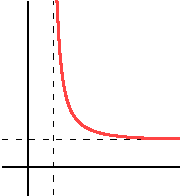
\includegraphics[scale=1]{zeta-function-real}
\end{wrapfigure}
Die Riemannsche~$\zeta$-Funktion ist also durch eine \emph{unendliche Reihe}
festgelegt. Je nachdem, wie schnell die Summanden einer unendlichen Reihe gegen
Null streben, hat sie entweder einen richtigen Zahlenwert (sie
\emph{konvergiert}), den Wert~$+\infty$ oder den Wert~$-\infty$ (sie
\emph{divergiert bestimmt}) oder gar keinen Wert (sie \emph{divergiert
unbestimmt}). Mit Reihen, die nicht konvergieren, kann man nicht wie gewöhnlich
rechnen -- das soll Aufgabe~\ref{aufg:grandi} demonstrieren. Mit dem
\emph{Integralvergleichskriterium}, das man im ersten Semester eines
Mathe-Studiums lernt, kann man aber leicht nachweisen, dass für~$s > 1$ die
gegebene Reihe konvergiert.

Der reelle Graph der~$\zeta$-Funktion ist recht unspektakulär. Er hat
die Geraden~$x = 1$ und~$y = 1$ als Asymptoten.
So unscheinbar dieser Graph und die Definition auch sein mögen, die Riemannsche~$\zeta$-Funktion
hat eine Vielzahl kurioser Eigenschaften und ist Gegenstand vieler
mathematischer Vermutungen. In der analytischen Zahlentheorie ist sie von
fundamentaler Bedeutung, angewendet wird sie aber auch in Physik,
Wahrscheinlichkeitstheorie und Statistik.

\begin{itemize}
\item Die~$\zeta$-Funktion lässt sich auch als ein zahlentheoretisches
interessantes Produkt schreiben (Abschnitt~\ref{sect:euler-produkt}).
\item Für~$s \to 1$ divergiert~$\zeta(s)$. Das ist eng mit der Unendlichkeit
der Primzahlen verbunden.
\item Es ist schwierig, geschlossene Ausdrücke für Funktionswerte
der~$\zeta$-Funktion anzugeben. Aber beispielsweise gilt~$\zeta(2) = \pi^2/6$.
Die Funktionswerte an allen anderen positiven geraden Zahlen~$n$ sind ebenfalls
bekannt, sie sind wie~$\zeta(2)$ bestimmte rationale Vielfache von~$\pi^n$.
\item Man vermutet, dass die Werte der~$\zeta$-Funktion an allen positiven
ungeraden Zahlen (außer der Eins) irrational sind. Man weiß schon, dass zumindest unendlich
viele dieser Werte irrational sind, und man weiß auch, dass~$\zeta(3)$
irrational ist. Es ist aber noch nicht einmal bekannt, ob auch~$\zeta(5)$ irrational
ist. (Kurioserweise weiß man aber, dass unter den Zahlen~$\zeta(5)$,
$\zeta(7)$, $\zeta(9)$ und~$\zeta(11)$ mindestens eine irrational sein muss.)
\item Obwohl die definierende Formel nur für~$s > 1$ konvergiert, lässt sich
die~$\zeta$-Funktion auf den Bereich~$s < 1$ und sogar auf \emph{alle komplexen
Zahlen} ungleich~$1$ fortsetzen.
\item Die Werte der~$\zeta$-Funktion an allen negativen ganzen Zahlen sind
bekannt. Bei allen negativen geraden Zahlen hat sie Nullstellen, die so
genannten \emph{trivialen Nullstellen der~$\zeta$-Funktion}.
\item Es ist bekannt, dass alle weiteren Nullstellen in den komplexen Zahlen
Realteil zwischen~$0$ und~$1$ (jeweils ausgeschlossen) haben.
\item Man vermutet, dass diese so genannten \emph{nichttrivialen Nullstellen}
sogar alle Realteil genau~$1/2$ haben. Das besagt die berühmte \emph{Riemannsche
Vermutung}.
\item Die Riemannsche Vermutung ist eng verwandt mit der Verteilung der
Primzahlen und der Goldbachschen Vermutung. Eine lange Liste von Konsequenzen
der Riemannschen Vermutung gibt es auf
\url{http://mathoverflow.net/questions/17209/consequences-of-the-riemann-hypothesis}.
\end{itemize}

\begin{aufgabe}{Eine einfache konvergente Reihe}\label{aufg:konvergente-reihen}
\begin{enumerate}
\item Was ergibt~$1 + 0{,}1 + 0{,}01 + 0{,}001 + \cdots$?
\item Was ergibt~$1 + 0{,}1_2 + 0{,}01_2 + 0{,}001_2 + \cdots$, wenn man die
Summanden im Binärsystem liest?
\end{enumerate}\fixlistspacing
\end{aufgabe}

\begin{aufgabe}{Grandis Reihe}\label{aufg:grandi}
Sei~$s \defeq 1 - 1 + 1 - 1 + \cdots$. Diese Reihe divergiert, man kann mit ihr
nicht wie gewöhnlich rechnen. Das sollen die folgenden Teilaufgaben
illustrieren. Die Reihe ist nach dem italienischen Mathematiker und
Geistlichen Guido Grandi (*~1671, †~1742) benannt.
\begin{enumerate}
\item Fasse die ersten beiden Summanden zusammen, dann die zweiten beiden, die
dritten beiden, und so weiter. Welches Ergebnis erhält man auf diese Art und
Weise für~$s$?
\item Lass den ersten Summanden vorne stehen, fasse dann aber den zweiten und
dritten Summanden zusammen, den vierten und fünften, und so weiter. Was
ist nun das Ergebnis?
\item Wie muss man die Summanden zusammenfassen, um deine Lieblingszahl als
Ergebnis zu erhalten?
\item Finde einen Weg, um die Gleichung~$1 - s = s$ nicht unplausibel zu
finden. Welchen Wert hat~$s$ dieser Gleichung zufolge?
\end{enumerate}\fixlistspacing
\end{aufgabe}

\begin{aufgabe}{Was ist~$\zeta(2)$?}\label{aufg:zeta2}
Die Zahl~$\zeta(2)$ ist gleich~$\pi^2/6$. Der übliche Beweis dieser Tatsache
verwendet mehrdimensionale Integrationstheorie und erfordert daher mehr
Vorkenntnisse, als wir hier voraussetzen möchten. Es ist aber auch schon spannend
zu verstehen, wieso~$\zeta(2)$ überhaupt \emph{endlich} ist. Das ist ja,
angesichts der Definition von~$\zeta(2)$ als die unendliche Reihe
\[ \zeta(2) = \frac{1}{1} + \frac{1}{4} + \frac{1}{9} + \frac{1}{16} + \cdots,
\]
gar nicht klar.
\begin{enumerate}
\item Finde zunächst den Wert von
\[ \sum_{n=2}^\infty \frac{1}{(n-1) \cdot n} =
  \frac{1}{1 \cdot 2} + \frac{1}{2 \cdot 3} + \frac{1}{3 \cdot 4} + \cdots. \]

\emph{Tipp.} Rechne nach, dass gilt: $\frac{1}{(n-1) \cdot n} = \frac{1}{n-1} -
\frac{1}{n}$. Mit dieser Erkenntnis kannst du die Summe umschreiben und
ausrechnen. Dabei wirst du feststellen, dass sich die meisten Summanden
gegenseitig wegheben. Summen, bei denen das passiert, heißen auch
\emph{Teleskopsummen}.

\item Zeige: $\zeta(2) < \infty$.

\emph{Tipp.} In welchem Größenverhältnis stehen~$\frac{1}{n^2}$
und~$\frac{1}{(n-1) \cdot n}$ zueinander?
\end{enumerate}

\emph{Bemerkung.} Eine Möglichkeit, den exakten Zahlenwert von~$\zeta(2)$ zu
bestimmen, zeigt folgende Rechnung auf.
\begin{align*}
  \zeta(2) &=
  \sum_{n=1}^\infty \frac{1}{n} \cdot \frac{1}{n} =
  \sum_{n=1}^\infty \Bigl(\int_0^1 x^{n-1} \,dx\Bigr) \cdot
    \Bigl(\int_0^1 y^{n-1} \,dy\Bigr) \\
  &=
  \sum_{n=1}^\infty \int_0^1 \int_0^1 x^{n-1} y^{n-1} \,dx\,dy
  = \int_0^1 \int_0^1 \sum_{n=1}^\infty x^{n-1} y^{n-1} \,dx\,dy \\
  &= \int_0^1 \int_0^1 \sum_{i=0}^\infty (xy)^i \,dx\,dy
  \stackrel{\text{A\ref{aufg:geometrische-reihe}}}{=} \int_0^1 \int_0^1 \frac{1}{1 - xy} \,dx\,dy
\end{align*}
Dabei ist insbesondere zu begründen, dass die unendliche Summe mit dem Integral
vertauscht werden kann. Das mehrdimensionale Integral am Ende muss
dann noch ausgewertet werden, zum Beispiel über eine trickreiche
Koordinatentransformation.
\end{aufgabe}


\section{Die Eulersche Produktformel}\label{sect:euler-produkt}

\begin{thm}Für alle~$s > 1$ gilt die Identität
\[ \zeta(s) = \bigprod_{\substack{p\\\prim{p}}} \frac{1}{1 - p^{-s}} =
  \frac{1}{1 - 2^{-s}} \cdot \frac{1}{1 - 3^{-s}} \cdot \frac{1}{1 - 5^{-s}} \cdots. \]
\end{thm}
Diese Beziehung ist aus mehreren Gründen bemerkenswert. Zunächst einmal ist es
eine Seltenheit, dass sich eine \emph{Summe} (die linke Seite der Gleichung)
auch als ein (nichttriviales) \emph{Produkt} schreiben lässt. Zudem noch gehen
in die rechte Seite die Primzahlen ein, beim bloßen Anblick der Formel für
die~$\zeta$-Funktion würde man das nicht vermuten.

Für den Beweis benötigen wir die Formel für die \emph{geometrische Reihe}
(Aufgabe~\ref{aufg:geometrische-reihe}),
\[ \sum_{m = 0}^\infty x^m = 1 + x + x^2 + x^3 + \cdots = \frac{1}{1 - x}, \]
und die Potenzgesetze~$x^{-a} = 1/x^a$ sowie~$(x^a)^b = x^{ab}$.

\begin{proof}Wir beginnen mit der rechten Seite der Gleichung. Der Bruch passt
auf die Formel für die geometrische Reihe, deswegen gilt
\[
  \bigprod_{\substack{p\\\prim{p}}} \frac{1}{1 - p^{-s}} =
  \bigprod_{\substack{p\\\prim{p}}} \left(1 + p^{-s} + (p^2)^{-s} + \cdots\right).
\]
Wenn wir dieses unendliche Produkt ausmultiplizieren, erhalten wir
die Summe über alle Zahlen der Form~$1/t^s$, wobei~$t$ alle Möglichkeiten,
beliebig viele Primzahlen aufzumultiplizieren, durchläuft. Da sich nach dem
Fundamentalsatz der Arithmetik jede positive natürliche Zahl auf genau eine Art
und Weise als Produkt von Primzahlen schreiben lässt, erhalten wir also die
Summe über alle Zahlen der Form~$1/n^s$, wobei~$n$ alle positiven natürlichen
Zahlen durchläuft. Nach Definition ist diese Summe~$\zeta(s)$.
\end{proof}

Überblick verloren? Aufgabe~\ref{aufg:euler-produkt} wird in kleinen handlichen
Stücken den Beweis verständlich machen.

\begin{aufgabe}{Die geometrische Reihe}\label{aufg:geometrische-reihe}
In dieser Aufgabe wollen wir die so genannte \emph{geometrishe Reihe}
\[ s \defeq 1 + x + x^2 + x^3 + \cdots \]
auswerten. Der erste Schritt dazu ist mit dieser Zeile schon getan -- in der
Mathematik wird vieles einfacher, wenn man dem Unbekannten einen Namen
gibt:~$s$. Denn dann steht der Weg für algebraische Umformungen offen.
\begin{enumerate}
\item Rechne nach: $s \cdot (1 - x) = 1$.

\emph{Tipp.} Multipliziere die unendliche Summe aus.

\item Folgere: $s = 1/(1-x)$.

\item Löse Aufgabe~\ref{aufg:konvergente-reihen} erneut, und zwar unter
Verwendung der Formel aus~b).
\end{enumerate}

\emph{Bemerkung.} Die Multiplikation mit~$(1-x)$, die zur Auswertung von~$s$
also sehr hilfreich war, war ein \emph{Trick}. Der Definition von~$s$ ist
dieser nicht zu entnehmen, man benötigt Kreativität und Geduld, um auf ihn zu
kommen. Die geometrische Reihe konvergiert nur, falls der Betrag von~$s$
kleiner als~$1$ ist, und nur in diesem Fall gilt die Formel~$s = 1/(1-x)$.
Diese Subtilitäten wollen wir nicht weiter beachten, obwohl sie durchaus
wichtig sind.
\end{aufgabe}

\begin{aufgabe}{Beweise ohne Worte}\label{aufg:ohne-worte}
Die aus dem Internet ausgeliehenen Skizzen demonstrieren (von links
nach rechts) folgende Sachverhalte -- und zwar ganz ohne
Formeln und Rechnungen. Schaue dir die Skizzen lang genug an, um zu verstehen,
wieso sie diese Sachverhalte wirklich beweisen.
\begin{multicols}{2}
\begin{enumerate}
\item $\frac{1}{4} + \left(\frac{1}{4}\right)^2 + \left(\frac{1}{4}\right)^3 +
\cdots = \frac{1}{3}$.
\item Wie bei~a).
\item $\frac{1}{3} + \left(\frac{1}{3}\right)^2 + \left(\frac{1}{3}\right)^3 +
\cdots = \frac{1}{2}$.
\item $\frac{1}{2} + \left(\frac{1}{2}\right)^2 + \left(\frac{1}{2}\right)^3 +
\cdots = 1$.
\end{enumerate}
\end{multicols}
\begin{center}
  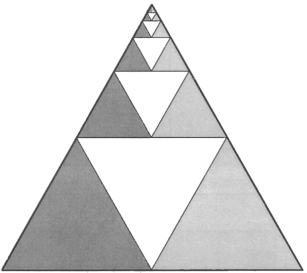
\includegraphics[height=0.2\textwidth]{geometrische-reihe-1}\quad
  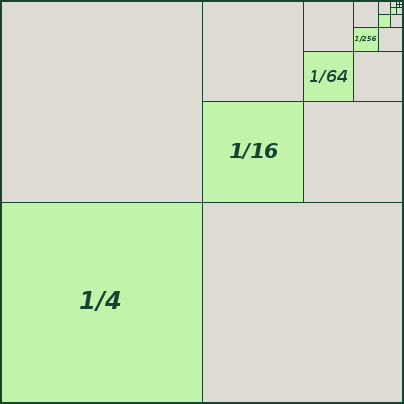
\includegraphics[height=0.2\textwidth]{geometrische-reihe-2}\quad
  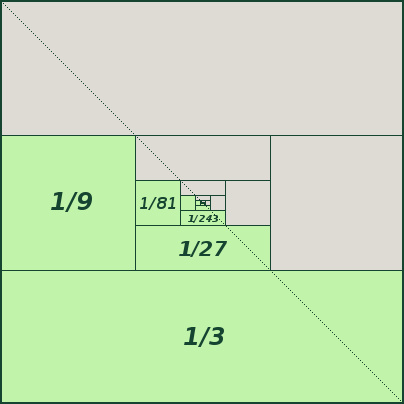
\includegraphics[height=0.2\textwidth]{geometrische-reihe-3}\quad
  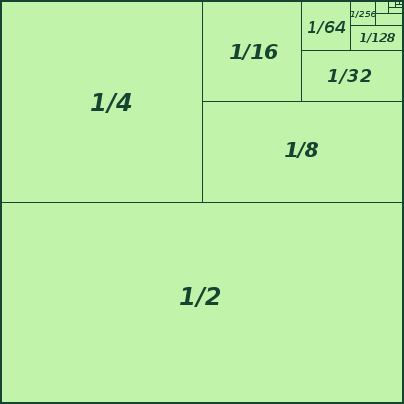
\includegraphics[height=0.2\textwidth]{geometrische-reihe-4}
\end{center}
Es ist sogar möglich, die allgemeine Formel für die geometrische Reihe aus
Aufgabe~\ref{aufg:geometrische-reihe} durch eine aussagekräftige Skizze zu
beweisen. Kannst du erklären, wie das funktioniert? (Achtung, knifflig!)
\begin{center}
  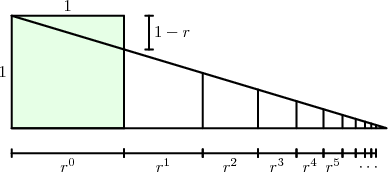
\includegraphics[scale=0.5]{geometrische-reihe-6}
\end{center}
\end{aufgabe}

\begin{aufgabe}{Die Eulersche Produktformel in fünf Schritten}
\label{aufg:euler-produkt}
\begin{enumerate}
\item Zum Aufwärmen: Multipliziere folgendes Produkt aus.
\[ \left(1 + \frac{1}{2} + \frac{1}{2^2}\right) \cdot
  \left(1 + \frac{1}{3} + \frac{1}{3^2}\right). \]
\item Multipliziere jetzt in dem Produkt
\[ \left(1 + \frac{1}{2} + \frac{1}{2^2} + \frac{1}{2^3} + \cdots\right) \cdot
  \left(1 + \frac{1}{3} + \frac{1}{3^2} + \frac{1}{3^3} + \cdots\right) \]
die Klammern so lange aus, bis du genug von dem System verstehst, um zu
erkennen: Hier kommt die Summe über die Kehrwerte von all den positiven
natürlichen Zahlen, in deren Primfaktorzerlegung nur die Faktoren~$2$ und~$3$
auftreten, heraus.
\item Multipliziere nun das dreifache Produkt
\[ \left(1 + \frac{1}{2} + \frac{1}{2^2} + \cdots\right) \cdot
  \left(1 + \frac{1}{3} + \frac{1}{3^2} + \cdots\right) \cdot
  \left(1 + \frac{1}{5} + \frac{1}{5^2} + \cdots\right) \]
soweit aus, um zu erkennen, dass das die Summe über die Kehrwerte von all den
positiven natürlichen Zahlen, in deren Primfaktorzerlegung nur die Faktoren~$2$,~$3$
und~$5$ vorkommen, ergibt.
\item Mit dieser Vorarbeit ist es nicht mehr schwer, zu glauben, dass das
unendliche Produkt
\[ \left(1 + \frac{1}{2} + \frac{1}{2^2} + \cdots\right)
  \left(1 + \frac{1}{3} + \frac{1}{3^2} + \cdots\right)
  \left(1 + \frac{1}{5} + \frac{1}{5^2} + \cdots\right) \cdots \]
gleich der Summe über die Kehrwerte von \emph{allen} positiven natürlichen Zahlen ist.
\item Schlussendlich: Ergänzen wir überall ein "`hoch~$s$"', so erhalten wir
die Summe über alle Zahlen der Form~$1/n^s$, wobei~$n$ über alle positiven
natürlichen Zahlen läuft. Das ist die Eulersche Produktformel.
\[\textstyle \left(1 + \frac{1}{2^s} + \frac{1}{(2^2)^s} + \cdots\right)
  \left(1 + \frac{1}{3^s} + \frac{1}{(3^2)^s} + \cdots\right)
  \left(1 + \frac{1}{5^s} + \frac{1}{(5^2)^s} + \cdots\right) \cdots =
  \sum_{n=1}^\infty \frac{1}{n^s}. \]
\end{enumerate}\fixlistspacing
\end{aufgabe}

\begin{aufgabe}{Nullstellen der~$\zeta$-Funktion rechts von der Eins}
Die Nullstellen der~$\zeta$-Funktion spielen in der Zahlentheorie eine große
Rolle und sind Gegenstand der Riemannschen Vermutung. In dieser Aufgabe wollen
wir zwei erste Schritte in diese Richtung gehen.
\begin{enumerate}
\item Zeige, dass für alle reellen Zahlen~$s > 1$ die Zahl~$\zeta(s)$ ungleich
Null ist.
\item Zeige, dass auch für alle komplexen Zahlen~$s$ mit Realteil größer
als~Eins die Zahl~$\zeta(s)$ ungleich Null ist.

\emph{Hinweis.} Ist~$s$ komplex, so können die Summanden in der definierenden
Reihe für~$\zeta(s)$ unübersichtliche komplexe Zahlen werden, mit Real- und
Imaginärteilen, die sowohl positiv als auch negativ sein können. Verwende also
nicht die Reihendarstellung für~$\zeta(s)$, um diese Aufgabe zu lösen.
\end{enumerate}

\emph{Warnung.} Es stimmt auch, dass~$\zeta(s)$ für komplexe Zahlen~$s$ mit
Realteil genau gleich Eins nicht Null ist -- diese Tatsache ist äquivalent zum
Primzahlsatz (Theorem~\ref{thm:primzahlsatz}). Das kann man aber weder mit der
Reihendarstellung noch mit der Eulerschen Produktformel zeigen, denn diese
konvergieren nur für Realteil größer als Eins.
\end{aufgabe}

\begin{aufgabe}{Ein mathematisches Wunder}
Folgende bemerkenswerte Gleichung stellt einen Zusammenhang zwischen den
Quadratzahlen der Primzahlen und der Kreiszahl~$\pi$ her:
\[ \frac{3}{4} \cdot \frac{8}{9} \cdot \frac{24}{25} \cdot \frac{48}{49} \cdot
\frac{120}{121} \cdot \frac{168}{169} \cdot \ldots = \frac{6}{\pi^2}. \]
Der belgische Mathematiker Luc Lemaire meint dazu: "`Irgendein zum Scherzen
aufgelegter Gott der Mathematik hat die Kreislänge in der a priori völlig
unverwandten Liste der Primzahlen kodiert."'\footnotemark

Beweise diese Gleichung, indem du die Produktformel und das Ergebnis~$\zeta(2) =
\pi^2/6$ (diskutiert in Aufgabe~\ref{aufg:zeta2}) verwendest.
\end{aufgabe}
\footnotetext{Englisches Original:
``It means in particular that some facetious god of mathematics has encoded the
length of a circle in the list of prime numbers, totally unrelated a priori.''
\href{http://www.ems-ph.org/journals/newsletter/pdf/2004-12-54.pdf}{Luc
Lemaire, Mathematics is alive and well and thriving in Europe, Heft 54 des
Newsletter der European Mathematical Society, 2004.}}


\section{Die harmonische Reihe}
\label{sect:harmonische-reihe}

Die unendliche Reihe
\[ \frac{1}{1} + \frac{1}{2} + \frac{1}{3} + \frac{1}{4} + \cdots \]
wird \emph{harmonische Reihe} genannt. Sie divergiert bestimmt, ihr Wert
ist~$+\infty$.\enlargethispage{1em}

Mit ein wenig Hintergrundwissen aus Integrationstheorie kann man sich
überlegen, dass die harmonische Reihe in etwa so schnell wächst wie der
natürliche Logarithmus:
\begin{equation}
  \label{star}
  \tag{$\star$}
  \frac{1}{1} + \frac{1}{2} + \cdots + \frac{1}{n} \approx \ln(n),
\end{equation}
und eine verfeinerte Analyse liefert folgendes Resultat.

\begin{thm}Es gibt eine Konstante~$\gamma \approx 0{,}57722$, die
\emph{Euler--Mascheroni-Konstante}, der sich die Differenzen aus linker und
rechter Seite von~\eqref{star} beliebig genau nähern. In Symbolen:
\[ \sum_{i=1}^n \frac{1}{i} - \ln(n) \xrightarrow{n \to \infty}
\gamma. \]
\end{thm}

In diesem Kontext gibt es eine Abschätzung, die für unsere Zwecke wichtig sein wird:
\[ \sum_{i=1}^{\lceil e^{A-\gamma} \rceil} \tfrac{1}{i} > A. \]
Die Klammern bezeichnen dabei die \emph{Aufrundungsoperation} (zur nächsten
ganzen Zahl).

\begin{center}\begin{tabular}{rrrr}
  \toprule
  $A$ & $e^{A-\gamma}$ & $\lceil e^{A-\gamma} \rceil$ & $\sum_{i=1}^{\lceil e^{A-\gamma} \rceil} 1/i$ \\\midrule
   1 &     1.56 &     2 &  1.50 \\
   2 &     4.23 &     5 &  2.28 \\
   3 &    11.50 &    12 &  3.10 \\
   4 &    31.26 &    32 &  4.06 \\
   5 &    84.97 &    85 &  5.03 \\
   6 &   230.97 &   231 &  6.02 \\
   7 &   627.84 &   628 &  7.02 \\
   8 &  1706.63 &  1707 &  8.02 \\
   9 &  4639.11 &  4640 &  9.02 \\
  10 & 12610.42 & 12611 & 10.02 \\
  \bottomrule
\end{tabular}\end{center}

\begin{aufgabe}{Divergenz der harmonischen Reihe}
\begin{enumerate}
\item Wieso ist~$\frac{1}{3} + \frac{1}{4} \geq \frac{1}{2}$?
\tabto{6cm}
\emph{Tipp.} $\frac{1}{3} \geq \frac{1}{4}$ und~$\frac{1}{4} + \frac{1}{4} =
\frac{1}{2}$.
\item Wieso ist~$\frac{1}{5} + \frac{1}{6} + \frac{1}{7} + \frac{1}{8} \geq \frac{1}{2}$?
\tabto{6cm}
\emph{Tipp.} $\frac{1}{5}, \frac{1}{6}, \frac{1}{7} \geq \frac{1}{8}$.

\item Wieso ist~$\frac{1}{9} + \cdots + \frac{1}{16} \geq \frac{1}{2}$?

\item Wieso ist~$\frac{1}{17} + \cdots + \frac{1}{32} \geq \frac{1}{2}$?

\item Folgere: Die harmonische Reihe ist größergleich
$\frac{1}{1} + \frac{1}{2} + \frac{1}{2} + \frac{1}{2} + \cdots$,
und das ist sicherlich~$+\infty$.
\end{enumerate}\fixlistspacing
\end{aufgabe}

\begin{aufgabe}{Slow harmonic series is slow}
Die harmonische Reihe divergiert zwar, tut das aber sehr langsam. Addiere mit
einem Taschenrechner oder einem Computerprogramm so viele Terme der Reihe, wie
du möchtest. Ich wette, du wirst nicht über~$30$ hinauskommen.
\end{aufgabe}

\begin{aufgabe}{Eulers Beweis der Unendlichkeit der Primzahlen}
\begin{enumerate}
\item Was ist~$\zeta(1)$?
\item Verwende Eulers Produktformel, um einen Beweis der
Unendlichkeit der Primzahlen zu führen: Wie sähe die Formel aus, wenn es nur
endlich viele Primzahlen gäbe?
\end{enumerate}\fixlistspacing
\end{aufgabe}


\section{Grobe Schranken für die Größen der Primzahlen}

Es gibt keine geschlossene Formel für die Primzahlen.\footnote{Das ist nur halb
wahr. Informiere dich über \emph{Mills Formel}.} Trotzdem kann man explizite
\emph{Schranken} für die Größe der~$n$-ten Primzahl angeben. Mit deren Hilfe
kann man bestimmen, wie viele Primzahlen es in einem vorgegebenem Bereich
mindestens geben muss oder höchstens geben kann.

Ein erstes Resultat in diese Richtung ist das folgende. Dabei
sei~$p_1,p_2,p_3,\ldots$ die unendliche Liste aller Primzahlen.

\begin{thm}\label{thm:schranke1}\ \\[-2em]
\begin{enumerate}
\item
Ist~$p$ eine Primzahl, so ist die nächste Primzahl kleiner oder gleich~$p! + 1$. \\[-2em]
\item
Die~$r$-te Primzahl ist höchstens~$2^{(2^r)}$: $p_r < 2^{(2^r)}$.
\end{enumerate}
\end{thm}

Das folgende Resultat ist schwieriger zu beweisen, liefert aber auch eine
bessere (kleinere) Abschätzung. Die Klammern bezeichnen wieder die
Aufrundungoperation.

\begin{thm}\label{thm:schranke2}\ \\[-2em]
\begin{enumerate}
\item
Ist~$p$ eine Primzahl, so ist die nächste Primzahl kleiner oder gleich~$\lceil e^{p-\gamma}
\rceil$. \\[-2em]
\item
Die~$r$-te Primzahl ist höchstens~$\lceil e^{r-\gamma} \rceil$: $p_r
\leq \lceil e^{r-\gamma} \rceil$.
\end{enumerate}
\end{thm}

Um diese beiden Behauptungen zu beweisen, werden wir eine interessante
mathematische Technik verwenden: \emph{Proof mining}. Deren Ausgangspunkt ist
die triviale Erkenntnis, dass ein \emph{Beweis} einer Aussage viel mehr enthält
als die bloße Information, dass die bewiesene Aussage korrekt ist. Ein Beweis
gibt auch (mehr oder weniger verständliche) Hintergründe zu ihrer Korrektheit,
knüpft Verbindungen zwischen unterschiedlichen mathematischen Objekten und
führt so Verborgenes auf Offensichtliches zurück.

Das führt dazu, dass man aus Beweisen rein qualitativer Aussagen -- zum
Beispiel: \emph{Es gibt unendlich viele Primzahlen.} -- oftmals quantitative
Information extrahieren kann: \emph{Im Bereich von~$1$ bis~$n$ gibt es
mindestens soundso viele Primzahlen.}

Proof mining werden wir an Euklids und an Eulers Beweis der Unendlichkeit der
Primzahlen üben. Euklids Beweis liefert Theorem~\ref{thm:schranke1}, Eulers
komplexerer Beweis liefert das stärkere Theorem~\ref{thm:schranke2}.

Beide Theoreme sind aber nur allererste Schritte im Verständnis der Asymptotik
der Primzahlen. Es gibt nämlich die beiden folgenden, viel schärferen Aussagen.
Wir werden sie später im Detail diskutieren.

\begin{thm}[Bertrands Postulat]Ist~$p$ eine Primzahl, so ist die nächste
Primzahl höchstens~$2p$.
\end{thm}

\begin{thm}[Primzahlsatz, ungenau formuliert]Zwischen~$1$ und~$n$ gibt es
etwa~$n/\ln n$ viele Primzahlen.\end{thm}

\begin{aufgabe}{Theorem~\ref{thm:schranke1} aus Euklids Beweis der
Unendlichkeit der Primzahlen}
\begin{enumerate}
\item Studiere Euklids Beweis der Unendlichkeit der Primzahlen
(Aufgabe~\ref{aufg:unendlich-euklid}), um zu sehen: Ist~$p$ eine Primzahl, so
kommt spätestens bis zu~$p! + 1$ ("`$p$ Fakultät"', $p! = 1 \cdot 2 \cdot
\ldots \cdot (p-1) \cdot p$) die nächste Primzahl.
\item Zeige: Für die~$(r+1)$-te Primzahl gilt die Abschätzung
\[ p_{r+1} \leq p_1 \cdots p_r + 1. \]
\item Folgere mit vollständiger Induktion:
\[ p_r < 2^{(2^r)}. \]

\emph{Tipp.} Verwende, dass für alle Zahlen~$m \geq 2$ gilt: $m/4 +
1 \leq m$. Verwende außerdem die Formel~$2^1 + 2^2 + \cdots + 2^k = 2^{k+1} -
2$.
\item Es gilt sogar~$p_r \leq \sqrt{2}^{(2^r)} = 2^{(2^{r-1})}$. Kannst du das
auch zeigen?
\end{enumerate}\fixlistspacing
\end{aufgabe}

\begin{aufgabe}{Theorem~\ref{thm:schranke2} aus Eulers Beweis der
Unendlichkeit der Primzahlen}
\begin{enumerate}
\item Sei~$q$ eine natürliche Zahl. Studiere den Beweis von Eulers
Produktformel, um folgende verfeinerte Aussage nachzuvollziehen:
\[ \bigsum_n \frac{1}{n} = \bigprod_{\substack{p \leq q \\ \prim{p}}} \frac{1}{1 -
p^{-1}}. \]
Die Summe auf der linken Seite soll dabei über all diejenigen positiven
natürlichen Zahlen laufen, in deren Primfaktoren nur Primzahlen~$\leq q$
vorkommen. Passend dazu läuft das Produkt auf der rechten Seite über alle
Primzahlen~$\leq q$.
\item Beweise:
\[
  \bigprod_{\substack{p \leq q \\ \prim{p}}} \frac{1}{1 - p^{-1}} =
  \bigprod_{\substack{p \leq q \\ \prim{p}}} \frac{p}{p - 1} \leq
  \bigprod_{a=1}^q \frac{a}{a - 1} = q. \]
\item Sei~$q$ eine Primzahl. Angenommen, bis zur Zahl~$\lceil e^{q-\gamma}
\rceil$ (einschließlich) kommen keine weiteren Primzahlen. Zeige dann
\[ \bigsum_{n=1}^{\lceil e^{q-\gamma} \rceil} \frac{1}{n} \leq q. \]
\item Verwende die Abschätzung aus Abschnitt~\ref{sect:harmonische-reihe}, um
zu sehen, dass das nicht sein kann und dass daher zwischen~$q+1$ und~$\lceil
e^{q-\gamma} \rceil$ mindestens eine weitere Primzahl liegen muss.
\item Beweise:
\[
  \bigprod_{i=1}^r \frac{1}{1 - p_i^{-1}} \leq
  \bigprod_{i=1}^r \frac{1}{1 - (i+1)^{-1}} =
  \bigprod_{i=1}^r \frac{i+1}{i} = r+1. \]
\item Folgere: Die~$(r+1)$-te Primzahl ist kleinergleich~$\lceil e^{r+1-\gamma} \rceil$.
\end{enumerate}\fixlistspacing
\end{aufgabe}


\section{Grobe Schranken für die Anzahl der Primzahlen}

In der Zahlentheorie interessieren wir uns für den Verlauf der
\emph{Primzahlfunktion}~$\pi$:
\begin{align*}
  \pi(n) &\defeq \text{Anzahl Primzahlen zwischen $1$ und $n$} \\
  &= \sum_{p \leq n} 1.
\end{align*}
Der gefeierte \emph{Primzahlsatz} gibt zwar keine explizite Formel für~$\pi(n)$,
macht aber sehr wohl eine Aussage über die \emph{Asymptotik} von~$\pi$. Er gibt
also eine Antwort auf die Frage, welchem Term sich~$\pi(n)$ für größer
werdendes~$n$ immer weiter annähert.

Im Graphen links sind gut die Sprünge bei den Primzahlen zu erkennen. Das etwas
chaotische Verhalten verschwindet, wenn man die Primzahlfunktion auf größeren
Skalen betrachtet (rechts).

\begin{center}
  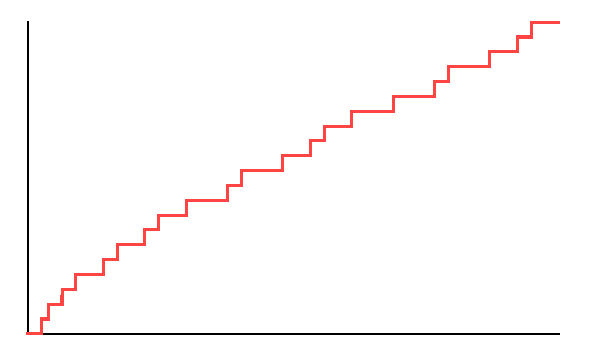
\includegraphics[scale=0.5]{pi-function-1}\qquad\qquad
  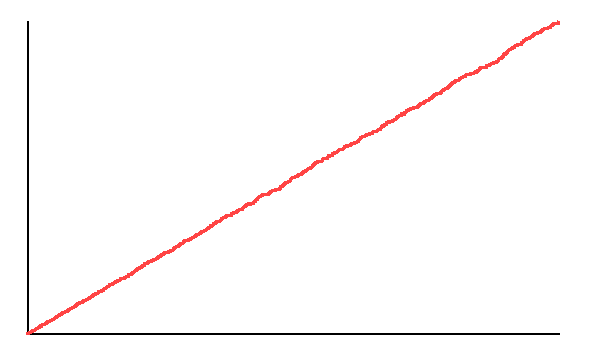
\includegraphics[scale=0.5]{pi-function-2}
\end{center}

\begin{thm}[Primzahlsatz]\label{thm:primzahlsatz}
Asymptotisch gilt
\[ \pi(n) \sim \frac{n}{\ln n}. \]
Genauer: Der Grenzwert für~$n \to \infty$ von~$\pi(n) / \frac{n}{\ln n}$ ist
Eins.
\end{thm}

Dieses Resultat wurde schon Ende des 18. Jahrhunderts von Gauß und Legendre
vermutet, konnte aber erst 1896 durch Hadamard und De La Vallée-Poussin rigoros
bewiesen werden. Wegweisend für den Beweis war eine Arbeit Riemanns aus dem
Jahr~1859 mit dem vielversprechenden Titel \emph{Über die Anzahl der Primzahlen
unter einer gegebenen Größe}. Wie der Beweis in etwa funktioniert, werden wir
noch verstehen. Die noch unbewiesene Riemannsche Vermutung impliziert übrigens
eine Verbesserung des Primzahlsatzes.

Um die Aussage des Primzahlsatzes besser wertschätzen zu können, möchten wir
zwei deutlich schwächere Abschätzungen angeben, die wir mit den Ergebnissen aus
dem vorherigen Abschnitt beweisen können. Dabei ist~$\ld$ der Logarithmus zur
Basis~$2$.

\begin{thm}\label{thm:pi-schranke1}$\pi(n) \geq \ld \ld n$.\end{thm}
\begin{thm}\label{thm:pi-schranke2}$\pi(n) \geq \ln n$.\end{thm}

\begin{center}
  \begin{tabular}{rrrrrr}
    \toprule
    $n$ & $\pi(n)$ & $n/\ln n$ & $\pi(n)/\frac{n}{\ln n}$ & $\ld\ld n$ & $\ln n$ \\\midrule
    10    & 4    &   4.3     & 0.921     & 1.7 & 2.3 \\
    100   & 25    &  21.7      & 1.151   &    2.7 & 4.6 \\
    1000  & 168    & 144.8     & 1.161   &   3.3 & 6.9 \\
    10000 & 1229   & 1085.7    &  1.132 & 3.7 &  9.2 \\
    100000  &  9592 &    8685.9      & 1.104 & 4.1 &  11.5 \\
    1000000 &      78498 &  72382.4     &  1.084 & 4.3 &  13.8 \\
    10000000 &     664579 & 620420.7    &   1.071 & 4.5 &  16.1 \\
    100000000 &    5761455 & 5428681.0  &     1.061 & 4.7 & 18.4 \\
    \bottomrule
  \end{tabular}
\end{center}

\begin{bem}Der Primzahlsatz behauptet nicht, dass der Unterschied
zwischen~$\pi(n)$ und~$\frac{n}{\ln n}$, also die Differenz~$\pi(n) - \frac{n}{\ln n}$, für~$n
\to \infty$ gegen Null geht. Tatsächlich strebt diese Differenz
gegen~$+\infty$. Der Primzahlsatz trifft eine Aussage über den \emph{relativen
Fehler}, also den Bruch~$(\pi(n)-\frac{n}{\ln n})/\pi(n)$. Dieser geht für~$n \to
\infty$ gegen Null.
\end{bem}


\begin{aufgabe}{Theorem~\ref{thm:pi-schranke1} aus Euklids Beweis der
Unendlichkeit der Primzahlen}
Aus Euklids Beweis haben wir die Abschätzung
\[ p_n < 2^{2^n} \]
extrahiert. Zeige damit für alle Primzahlen~$p$, dass~$\pi(p) > \ld \ld p$.

\emph{Tipp.} Es gilt~$\pi(p_n) = n$, wieso?

\emph{Hinweis.} Wenn du möchtest, kannst du versuchen, auch noch~$\pi(n) > \ld
\ld n$ für alle natürlichen Zahlen (statt nur für die Primzahlen) zu beweisen.
Die Hauptarbeit ist dabei schon erledigt, denn die linke Seite macht nur bei
Primzahlen Sprünge, und die rechte wächst zwar kontinuierlich, ändert sich bis
zur nächsten Primzahl aber stets um weniger als Eins. Diese letzte Teilaussage
ohne weitere Hilfsmittel, insbesondere ohne Bertrands Postulat, zu beweisen,
ist aber nicht ganz einfach.
\end{aufgabe}

\begin{aufgabe}{Theorem~\ref{thm:pi-schranke2} aus Eulers Beweis der
Unendlichkeit der Primzahlen}
Aus Eulers Beweis haben wir die Abschätzung
\[ p_n \leq \lceil e^{n-\gamma} \rceil \]
extrahiert; tatsächlich gilt sogar "`$<$"' statt nur~"`$\leq$"'. Beweise damit
für alle Primzahlen~$p$, dass~$\pi(p) > \gamma + \ln p > \ln p$.
\end{aufgabe}

% XXX: Tabelle


\section{Die Summe der Kehrwerte der Primzahlen}

Es gibt genauso viele Quadratzahlen wie Primzahlen, nämlich jeweils
\emph{abzählbar unendlich viele}. Intuitiv würde man trotzdem behaupten, dass
die Primzahlen dichter gesäht seien als die Quadratzahlen. Eine Möglichkeit,
den Unterschied mathematisch präzise zu verdeutlichen, besteht darin, die Summe
der Kehrwerte zu vergleichen:
\[ \frac{1}{1} + \frac{1}{4} + \frac{1}{9} + \frac{1}{16} + \cdots
  \quad\text{vs.}\quad
  \frac{1}{2} + \frac{1}{3} + \frac{1}{5} + \frac{1}{7} + \cdots \]
Wie wir nämlich in Aufgabe~\ref{aufg:zeta2} gesehen haben, hat die linke Reihe
einen endlichen Wert (nämlich $\pi^2/6$). Die rechte Reihe dagegen divergiert, sie hat
den Wert~$+\infty$. Das zeigt, dass die Kehrwerte der Quadratzahlen viel schneller
kleiner werden als die Kehrwerte der Primzahlen; umgekehrt formuliert: die
Quadratzahlen wachsen viel schneller an als die Primzahlen.

\begin{thm}Die Summe der Kehrwerte der Primzahlen ist unendlich:
$\frac{1}{2} + \frac{1}{3} + \frac{1}{5} + \cdots = \infty$.
\end{thm}
\begin{proof}Wenn wir das Resultat aus Aufgabe~\ref{aufg:div-sum-p} umstellen,
erhalten wir
\[ \bigsum_{p \leq N} \frac{1}{p} \geq \ln \bigsum_{n=1}^N \frac{1}{n} - C, \]
wobei~$C$ eine Konstante ist.
Auf der rechten Seite kommt also die harmonische Reihe vor, von der wir bereits
wissen, dass sie divergiert (Abschnitt~\ref{sect:harmonische-reihe}).
\end{proof}

\begin{aufgabe}{Die Summe der Kehrwerte der Primzahlen}\label{aufg:div-sum-p}
Zeige:
\[ \ln \bigsum_{n=1}^N \frac{1}{n} \leq \bigsum_{p \leq N} \frac{1}{p} + C, \]
wobei~$C$ eine bestimmte Konstante ist. Die Summe auf der rechten Seite soll
über alle Primzahlen~$p$ zwischen~$1$ und~$N$ gehen. Beginne dazu mit der
linken Seite und führe eine lange Abschätzungskette, die zum Schluss in der
rechten Seite mündet. Verwende folgende Zutaten:
\begin{itemize}
\item $\sum_{n=1}^N \frac{1}{n} \leq \sum_n \frac{1}{n}$, wobei die Summe auf
der rechten Seite über all diejenigen natürlichen Zahlen läuft, in deren
Primfaktorzerlegung nur Primzahlen~$\leq N$ vorkommen. Wieso stimmt das?
\item $\sum_n \frac{1}{n} = \prod_{p \leq N} \frac{1}{1 - p^{-1}}$. Warum gilt
das?
\item $\ln(1-x^{-1}) = \frac{1}{x} + \frac{1}{2x^2} + \frac{1}{3x^3} + \cdots$.
Diese Formel musst du nicht beweisen, sie ist eine so genannte
\emph{Taylorentwicklung}.
\item Trenne eine Summe der Form $\sum_{p \leq N} (\frac{1}{p} + {??})$ in zwei
Teile auf: $\sum_{p \leq N} \frac{1}{p} + \sum_{p \leq N} {??}$.
\item Sobald es sich anbietet, $\frac{1}{p^2}$ auszuklammern, mach das.
\item Verwende die Formel für die geometrische Reihe, um $1 + \frac{1}{p} +
\frac{1}{p^2} + \cdots$ zu vereinfachen.
\item Verwende zum Schluss das Ergebnis aus Aufgabe~\ref{aufg:zeta2}a).
\end{itemize}\fixlistspacing
\end{aufgabe}


\section{\texorpdfstring{Die Mangoldt-Funktion~$\boldsymbol{\Lambda}$}{Die
Mangoldt-Funktion~Λ}}

Die Mangoldt-Funktion~$\Lambda$ (benannt nach dem deutschen Mathematiker Hans
von Mangoldt, *~1854, †~1925 und notiert durch ein großes griechisches Lambda)
ist in der analytischen Zahlentheorie eine wichtige Funktion. Sie ist eng
verwandt mit der Primzahlfunktion~$\pi$ und mit der
Riemannschen~$\zeta$-Funktion. Außerdem kommt sie in der Definition der
\emph{Tschebyschow-Funktion} vor -- eine Funktion, die wie~$\pi$ die Anzahl der
Primzahlen misst, mit der man aber dank besserer Eigenschaften leichter umgehen
kann.

\begin{defn}Für Primzahlpotenzen~$n = p^k$ mit~$k \geq 1$ ist die
\emph{Mangoldt-Funktion}~$\Lambda$ definiert durch~$\Lambda(n) = \ln p$. Für
alle anderen natürlichen Zahlen ist~$\Lambda(n) = 0$.\end{defn}

Im Graphen sind die unzähligen Nullstellen von~$\Lambda$ (alle Zahlen, die
keine reinen Primzahlpotenzen sind) anhand der Lücken erkennbar.

\begin{center}
  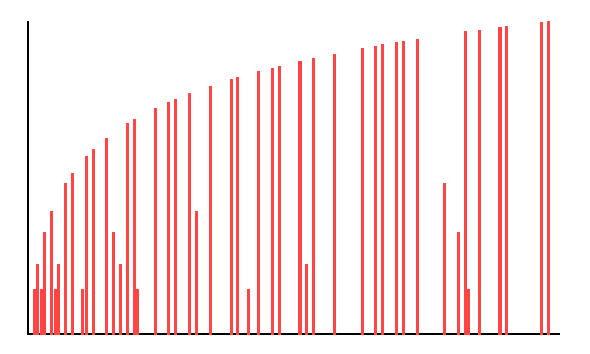
\includegraphics{mangoldt-function}
\end{center}

Ein erster Grund, wieso die Mangoldt-Funktion eine große zahlentheoretische
Bedeutung hat, zeigt das folgende Theorem.

\begin{thm}\label{thm:mangoldt-hauptsatz}Für jede positive natürliche Zahl~$n$
gilt
\[ \ln n = \sum_{d|n} \Lambda(d). \]
Dabei geht die Summe auf der rechten Seite über alle positiven Teiler von~$n$.
\end{thm}

Zum Beispiel sind die positiven Teiler von~$12$ die Zahlen~$1$, $2$, $3$, $4$,
$6$ und~$12$, und tatsächlich gilt, unter Verwendung der Rechenregel~$\ln(a
\cdot b) = \ln a + \ln b$ für Logarithmen:
\begin{align*}
  \ln 12 &= \ln(2 \cdot 2 \cdot 3) =
  \ln 2 + \ln 2 + \ln 3 =
  \Lambda(2) + \Lambda(4) + \Lambda(3) \\
  &= \Lambda(1) + \Lambda(2) + \Lambda(3) + \Lambda(4) + \Lambda(6) +
  \Lambda(12) \\
  &= \sum_{d|12} \Lambda(d).
\end{align*}

Den Zusammenhang zur Riemannschen~$\zeta$-Funktion stellt folgende Formel dar.

\begin{thm}\label{thm:mangoldt-zeta}
Die Ableitung von~$\zeta$, $\zeta$ selbst und~$\Lambda$ erfüllen
die Identität
\[ -\frac{\zeta'(s)}{\zeta(s)} = \sum_{n=1}^\infty \frac{\Lambda(n)}{n^s}. \]
\end{thm}

\begin{aufgabe}{Der Fundamentalsatz der Arithmetik in Mangoldt-Sprache}
Beweise Theorem~\ref{thm:mangoldt-hauptsatz}, zeige also für alle positiven
Zahlen~$n$, dass~$\ln n = \sum_{d|n} \Lambda(d)$.

\emph{Tipp.} Überlege dir anhand der Primfaktorzerlegung der Zahl~$n$, welche
Teiler~$n$ hat und welchen Wert die Mangoldt-Funktion~$\Lambda$ bei ihnen
annimmt. Erinnere dich außerdem an die Rechenregel~$\ln(a \cdot b) = \ln a +
\ln b$ für Logarithmen.
\end{aufgabe}

\begin{aufgabe}{Zusammenhang von~$\Lambda$ mit~$\zeta$}
Beweise Theorem~\ref{thm:mangoldt-zeta}.

\emph{Tipp.} Verwende die Eulersche Produktformel
(Abschnitt~\ref{sect:euler-produkt}), die Ableitungsregel~$(a^s)' = a^s \cdot
\ln a$ und die Produktregel für unendlich viele Faktoren:
\begin{align*}
  (f_1(s) \cdot f_2(s) \cdot f_3(s) \cdot \ldots)' &=
  f_1'(s) \cdot f_2(s) \cdot f_3(s) \cdot \ldots \\
  &\mathrel{+} f_1(s) \cdot f_2'(s) \cdot f_3(s) \cdot \ldots \\
  &\mathrel{+} f_1(s) \cdot f_2(s) \cdot f_3'(s) \cdot \ldots \\
  &\mathrel{+} \cdots.
\end{align*}
\vspace{-2em}
\end{aufgabe}

\begin{aufgabe}{Exkurs: Wieso das Zwölfersystem besser als das Zehnersystem ist}
Im Zwölfersystem verwendet man insgesamt zwölf Ziffern, nämlich die üblichen
Ziffern von~$0$ bis~$9$ und dann zwei neue Ziffern: $A$ für~$10$ und~$B$
für~$11$. Zum Beispiel steht die Zahl~$3B5_{12}$ für~$5$ Einer, $11$~Zwölfer
und~$3$ Vielfache von~144, also für die Zahl~$569$. Die Zahl~$2{,}2_{12}$ steht
für~$2$ Einer und~$2$ Zwölftel, also für~$2 + \frac{2}{12} =
2{,}1\overline{6}$.
\begin{enumerate}
\item Wie schreibt sich $1/3$ im Zwölfersystem?
\item Wie $1/4$ und $1/6$?
\item Wie $1/5$?
\item Welchen Vorteil hat also das Zwölfersystem gegenüber dem Zehnersystem? An
welcher Eigenschaft der Zahl~$12$ liegt das?
\end{enumerate}\fixlistspacing
\end{aufgabe}


\section{Asymptotische Notation}

\begin{defn}Sind~$f(x)$ und~$g(x)$ nichtnegative Funktionsterme, so schreiben
wir genau dann $f(x) \ll g(x)$ (in Worten: "`$f(x)$ ist asymptotisch kleiner
oder gleich~$g(x)$"'), wenn es eine Konstante~$C \geq 0$ gibt, sodass ab einer
gewissen Stelle~$x_0$ für alle~$x \geq x_0$ gilt, dass
\[ f(x) \leq C \cdot g(x). \]
\end{defn}

Auf Deutsch: Wenn wir~$f(x) \ll g(x)$ schreiben, meinen wir nicht, dass an
allen Stellen der Graph von~$f$ unterhalb von dem von~$g$ liegt. Wir meinen
stattdessen, dass -- ab einer gewissen Grenze, vorher dürfen~$f(x)$ und~$g(x)$
völlig beliebig verlaufen -- die Funktion~$f$ kleiner ist als irgendein
konstantes Vielfaches von~$g$. Um mit dieser Kurzschreibweise vertraut zu
werden, müssen wir uns ein paar Beispiele ansehen.

\begin{itemize}
\item $x \ll x^2$. Für~$x \in \left]0,1\right[$ ist zwar~$x$ größer als~$x^2$, danach aber
ist~$x$ kleiner als~$x^2$.
\item $100x \ll x^2$. Hier dauert es etwas länger, bis das stärkere Wachstum
der Quadratfunktion überwiegt.
\item $x^2 \ll x^2$. An diesem Beispiel sieht man, dass~"`$\ll$"' eine
asymptotische Variante von~"`$\leq$"', und nicht etwa von~"`$<$"' ist.
\item $3x^2 \ll x^2$. Es ist~$3x^2$ zwar nie kleiner als~$x^2$,
aber kleiner als ein bestimmtes konstantes Vielfaches von~$x^2$, nämlich zum
Beispiel dem Zehnfachen von~$x^2$.
\item $x^3 \not\ll x^2$. Die Kubikfunktion wächst stärker als die
Quadratfunktion, und sie wächst auch stärker als jedes konstante Vielfache der
Quadratfunktion.
\item $\arctan(x) \ll 1$. Im Grenzwert für~$x \to \infty$ strebt~$\arctan(x)$
gegen~$\pi/2 \approx 1{,}6$. Das ist zwar nicht kleiner als Eins, aber kleiner
als ein konstantes Vielfaches der Eins.
\item $1/x \ll x$. Für kleine~$x$ ist~$1/x$ viel größer als~$x$. Ab der
Stelle~$1$ jedoch ist~$1/x$ kleiner als~$x$.
\end{itemize}

\begin{lemma}\label{lemma:asympt}\begin{enumerate}
\item Wenn~$f(x) \ll g(x)$ und~$g(x) \ll h(x)$, dann auch~$f(x) \ll h(x)$.
\item Wenn~$f(x) \ll g(x)$ und~$a(x) \ll b(x)$, dann auch~$f(x)+a(x) \ll
g(x)+b(x)$.
\item Wenn~$f(x) \ll g(x)$ und~$a(x) \ll b(x)$, dann auch~$f(x) \cdot a(x) \ll
g(x) \cdot b(x)$.
\end{enumerate}
\end{lemma}

\begin{aufgabe}{Weitere Beispiele zur asymptotischen Notation}
\begin{wrapfigure}{r}{0.25\textwidth}
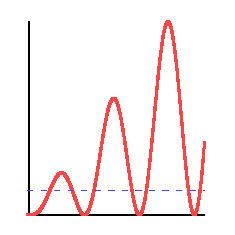
\includegraphics[width=3cm]{asymptotic-notation}
\end{wrapfigure}
\ \\
\vspace{-3em}
\begin{enumerate}
\item Gilt~$e^5 \ll x^5$ oder $x^5 \ll e^5$?
\item Gilt~$x \cdot \ln x \ll x$ oder $x \ll x \cdot \ln x$?
\item Gilt~$x \cdot \sin(x)^2 \ll x^5$?
\item Erkläre, wieso \emph{weder} $x \cdot \sin(x)^2 \ll 1$ \emph{noch} $1 \ll x
\cdot \sin(x)^2$ stimmt (siehe Skizze).
\end{enumerate}\fixlistspacing
\end{aufgabe}

\begin{aufgabe}{Theorie zur asymptotischen Notation}
Beweise Lemma~\ref{lemma:asympt}. Für Behauptung~a) kannst du dabei nach
folgendem Muster vorgehen; es sind nur noch die Lücken auszufüllen.

Da~$f(x) \ll g(x)$, gibt es eine Konstante~$C \geq 0$ und eine Schranke~$x_0$,
sodass für alle~$x \geq x_0$ gilt: $f(x) \leq C \cdot g(x)$. Da~$g(x) \ll
h(x)$, gibt es eine weitere Konstante~$D \geq 0$ und eine weitere
Schranke~$x_1$, sodass für alle~$x \geq x_1$ gilt: $g(x) \leq D \cdot h(x)$.
Daher gilt zusammengenommen für alle~$x \geq {??}$, dass~$f(x) \leq {??} \cdot
h(x)$. Also~$f(x) \ll h(x)$.
\end{aufgabe}

\begin{aufgabe}{Asymptotik und Grenzwerte}\label{aufg:asymp-limes}
Gelte, dass~$f(n) / g(n)$ für~$n \to \infty$ gegen eine Zahl~$a < \infty$
konvergiert. Überlege dir, dass dann~$f(n) \ll g(n)$.

\emph{Tipp.} Wenn~$\lim_{n \to \infty} \frac{f(n)}{g(n)} = a$, dann gibt es
irgendeine Stelle~$n_0$, sodass für alle~$n \geq n_0$ gilt: $f(n)/g(n) \leq
a+1$.
\end{aufgabe}


\section{\texorpdfstring{Die Tschebyschow-Funktion~$\boldsymbol{\psi}$}{Die
Tschebyschow-Funktion~ψ}}

\begin{defn}Die (zweite) \emph{Tschebyschow-Funktion}~$\psi$ ist definiert als
\[ \psi(x) \defeq \sum_{n \leq x} \Lambda(n). \]
Dabei geht die Summe über alle natürlichen Zahlen~$n \leq x$.\end{defn}

\begin{wrapfigure}{r}{0.3\textwidth}
  \vspace{-2em}
  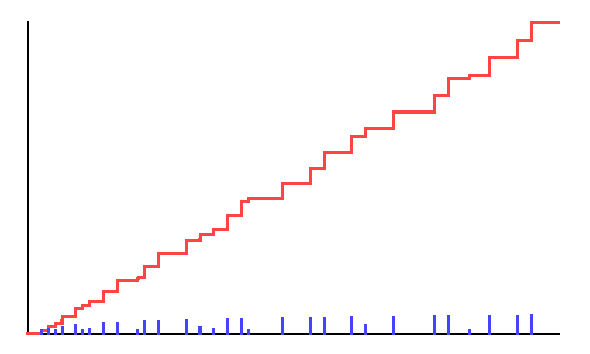
\includegraphics[width=0.25\textwidth]{chebyshev-function}
\end{wrapfigure}
Im Graphen (obere Kurve, in Rot) sind die Sprünge der Tschebyschow-Funktion bei
den Primzahlen und ihren Potenzen gut erkennbar. Zum Vergleich ist die Mangoldt-Funktion in Blau
eingezeichnet.

Unmittelbar sind wir eigentlich nicht an der Tschebyshow-Funktion, sondern an
der Primzahlfunktion~$\pi$ interessiert. Die beiden Funktionen sind aber eng
miteinander verwandt: Bei der Primzahlfunktion wird bei jeder neuen
Primzahl~$p$ der konstante Summand~$1$ addiert. Bei der Tschebyschow-Funktion
dagegen wird der Summand~$\ln p$ addiert, und außerdem wird~$\ln p$ auch bei
allen Potenzen von~$p$ addiert.

Das folgende Theorem zeigt, dass man den Primzahlsatz, der eine asymptotische
Aussage über~$\pi(n)$ trifft, auch auf~$\psi(n)$ umformulieren kann.

\begin{thm}\label{thm:psi-pi}
Sollte~$\psi(n)/n$ im Grenzwert~$n \to \infty$ den Wert~$1$ annehmen, so nimmt
auch~$\pi(n)/\frac{n}{\ln n}$ im Grenzwert den Wert~$1$ an; und umgekehrt.
\end{thm}

Der Primzahlsatz (Theorem~\ref{thm:primzahlsatz}) ist also äquivalent zur
Aussage, dass~$\psi(n)$ asymptotisch äquivalent zu~$n$ ist. Es hat sich
herausgestellt, dass es leichter ist, den Primzahlsatz über diesen Umweg mit
der Tschebyschow-Funktion als direkt zu beweisen.

Bevor wir uns im nächsten Abschnitt einem Beweis des Primzahlsatzes stellen,
möchten wir in diesem Abschnitt eine schwächere, aber immer noch interessante
Aussage verstehen.

\begin{thm}\label{thm:psi-obere-schranke}
Asymptotisch ist~$\psi(N)$ kleiner als~$N$: $\psi(N) \ll N$.
\end{thm}

\begin{proof}Der Beweis folgt in voneinander unabhängigen Schritten, die wir in
den folgenden Aufgaben bearbeiten.
\begin{itemize}
\item Um das Theorem zu beweisen, genügt es nachzuweisen, dass~$\sum_{N < n
\leq 2N} \Lambda(n) \ll N$.
\item In der Summe~$\sum_{N < n \leq 2N} \Lambda(n) = \Lambda(N+1) +
\Lambda(N+2) + \cdots + \Lambda(2N)$ untersuchen wir separat folgende Arten von
Summanden~$\Lambda(n)$: die, für die~$n$ eine Primzahlpotenz der Form~$p^j$
mit~$j \geq 2$ ist; die, für die~$n$ eine Primzahl ist; und alle restlichen
Zahlen.
\item Die Summe über die Summanden der ersten Art ist~$\ll N$.
\item Die Summe über die Summanden der zweiten Art ist~$\ll N$.
\item Die Summe über die Summanden der dritten Art ist Null und daher erst
recht~$\ll N$. \qedhere
\end{itemize}
\end{proof}

\begin{aufgabe}{Beweis von Theorem~\ref{thm:psi-obere-schranke}, Teil I:
Reduktionsschritt}
Nimm an, dass schon bewiesen wurde, dass
\[ \sum_{N < n \leq 2N} \Lambda(n) \ll N. \]
Dabei geht die Summe über alle natürlichen Zahlen zwischen~$N$ (ausschließlich)
und~$2N$ (einschließlich). Zeige unter dieser Annahme, dass dann auch
\[ \psi(N) = \sum_{n \leq N} \Lambda(n) \ll N. \]
Hierbei geht die Summe über alle natürlichen Zahlen~$\leq N$.

\emph{Tipp.} Zerlege die Summe~$\psi(N)$ in mehrere Teilbereiche:
von~$N/2$ bis~$N$; von~$N/4$ bis~$N/2$; von~$N/8$ bis~$N/4$; und so weiter.
Wende die Annahme auf jeden dieser Teilbereiche an und erinnere dich, dass~$1 +
1/2 + 1/4 + 1/8 + \cdots = 2$ (Aufgabe~\ref{aufg:ohne-worte}).
\end{aufgabe}

\begin{aufgabe}{Beweis von Theorem~\ref{thm:psi-obere-schranke}, Teil II:
Summanden erster Art}
In dieser Aufgabe betrachten wir in der Summe~$\sum_{N < n \leq 2N} \Lambda(n)$
all diejenigen Summanden, die zu Zahlen~$n$ der Form~$n = p^j$ mit einer Primzahl~$p$
und~$j \geq 2$ gehören (im Folgenden "`Summanden erster Art"' genannt).
\begin{enumerate}
\item Zeige: Eine solche Primzahl~$p$ ist~$\leq \sqrt{2N}$.
\item Folgere: Von den Summanden dieser Art gibt es höchstens~$\sqrt{2N}$ viele.
\item Mache dir klar, dass der Exponent~$j$ eines solchen Summanden
höchstens~$j_\text{max} \defeq \log_p(2N)$ ist.
\item Der Beitrag der Primzahl~$p$ zu Summanden dieser Art ist daher höchstens
$\ln p \cdot (j_\text{max}-2)$ (wieso?). Zeige, dass dieser
Beitrag höchstens $\ln(2N)$ ist.

\emph{Tipp.} Verwende das Logarithmusgesetz~$\log_p(2N) = \ln(2N)/\ln(p)$.
\item Folgere: Der Gesamtbeitrag aller Summanden erster Art ist höchstens
$\sqrt{2N} \cdot \ln(2N)$.
\item Beweise, dass diese obere Grenze~$\ll N$ ist.

\emph{Hinweis.} Wenn du bis zu dieser Stelle gekommen bist, hast du vielleicht
keine Lust mehr auf Rechnungen. Dann skizziere einfach~$\sqrt{2N} \cdot \ln(2N)
/ N$ (zum Beispiel auf WolframAlpha.com) und ermittle empirisch
den Grenzwert für~$N \to \infty$. Aufgabe~\ref{aufg:asymp-limes} verrät dir
dann, dass mehr nicht zu tun ist.
\end{enumerate}\fixlistspacing
\end{aufgabe}

\begin{aufgabe}{Beweis von Theorem~\ref{thm:psi-obere-schranke}, Teil III:
Summanden zweiter Art}
Es geht nun um die Summanden der Form~$\Lambda(p)$ in~$\sum_{N < n \leq 2N}
\Lambda(n)$, wobei~$p$ eine Primzahl zwischen~$N$ (ausschließlich) und~$2N$
(einschließlich) ist ("`Summanden zweiter Art"'). Die folgenden Teilaufgaben
können unabhängig voneinander bearbeitet werden.
\begin{enumerate}
\item Beweise, dass eine solche Primzahl~$p$ den
Binomialkoeffizienten~$\binom{2N}{N}$ teilt. Verwende dazu folgende Formel:
\[ \binom{2N}{N} = \frac{(2N)!}{N! \cdot N!} =
  \frac{(2N) \cdot (2N-1) \cdot \ldots \cdot 2 \cdot 1}{
  N \cdot (N-1) \cdot \ldots \cdot 2 \cdot 1 \cdot
  N \cdot (N-1) \cdot \ldots \cdot 2 \cdot 1} \]
\item Folgere, dass das Produkt aller Primzahlen zwischen~$N$
(ausschließlich) und~$2N$ (einschließlich) die Zahl~$\binom{2N}{N}$ teilt.
\item Beweise: Der Gesamtbeitrag der Summanden zweiter Art, also~$\sum_{N < p
\leq 2N} \ln p$, ist höchstens~$\ln 2^{2N}$.

\emph{Hinweis.} Es gilt~$\binom{2N}{N} \leq 2^{2N}$. Das zeigt die folgende
Aufgabe.
\item Beweise, dass~$\ln 2^{2N} \ll N$.
\end{enumerate}\fixlistspacing
\end{aufgabe}

\begin{aufgabe}{Eine Abschätzung für Binomialkoeffizienten}
In dieser Aufgabe wollen wir folgende Abschätzung beweisen:
\[ \binom{n}{k} = \frac{n!}{k! \cdot (n-k)!} \leq 2^n. \]
\begin{enumerate}
\item Erkläre, wieso es~$2^n$ viele Teilmengen der Menge~$\{1,\ldots,n\}$ gibt
-- die leere Teilmenge und ganz~$\{1,\ldots,n\}$ mitgezählt.
\item In der Kombinatorik lernt man, dass~$\binom{n}{k}$ die Anzahl der
\emph{$k$-elementigen} Teilmengen der Menge~$\{1,\ldots,n\}$ ist. Wieso genügt
diese Einsicht in Kombination mit Teilaufgabe~a), um die Abschätzung zu
beweisen?
\end{enumerate}
Es gibt auch einen rechnerischen Beweis der Abschätzung. Und zwar besagt
der \emph{binomische Lehrsatz}, dass
\begin{align*}
  (x+y)^n &= \textstyle \binom{n}{0} x^n + \binom{n}{1} x^{n-1} y
  + \binom{n}{2} x^{n-2} y^2 +
  \cdots
  +
  \binom{n}{n-2} x^2 y^{n-2} +
  \binom{n}{n-1} x y^{n-1} +
  \binom{n}{n} y^n.
\end{align*}
Für~$n = 2$ erhält man aus dieser Formel die bekannte erste binomische Formel,
\begin{align*}
  (x+y)^2 &= x^2 + 2xy + y^2, \\
\intertext{und für~$n = 3$ erhält man}
  (x+y)^3 &= x^3 + 3x^2y + 3xy^2 + y^3.
\end{align*}
\begin{enumerate}
\addtocounter{enumi}{2}
\item Schreibe~$2^n$ als~$(1 + 1)^n$ und führe damit einen Beweis der
Abschätzung über den binomischen Lehrsatz.
\end{enumerate}\fixlistspacing
\end{aufgabe}


\section{Weitere Stichpunkte}

Ausblick in Stichpunkten, muss noch ausgeführt werden:
\begin{itemize}
\item Zusammenhang zwischen~$\pi$ und~$\psi$
\item Beweis, dass~$\pi(x) \ll x/\ln x$
\item Beweis, dass der Primzahlsatz äquivalent dazu ist, dass die
Riemannsche~$\zeta$-Funktion keine Nullstellen mit Realteil~1 hat
\item Beweis, dass die Riemannsche~$\zeta$-Funktion keine Nullstellen mit
Realteil~1 hat, unter Verwendung einer expliziten Formel für~$\Lambda(n)$, in
der die Nullstellen von~$\zeta$ vorkommen
\item Erklärung, inwieweit die Nullstellen der~$\zeta$-Funktion wie Klänge
sind; und Erklärung, inwieweit die Riemannsche Vermutung impliziert, dass die
Nullstellen sogar einen Akkord bilden (auf Terence Tao verweisen)
\item Erklärung, inwieweit sich Primzahlen wie Zufallszahlen verhalten; und
Erklärung, inwieweit sie das nicht tun
\item Erklärung, in welchem Sinn~$1 + 2 + 3 + \cdots = -1/12$ gilt; und was das mit
dem Casimir-Effekt aus der Physik zu tun hat
\end{itemize}

\end{document}

Casimir-Effekt
Riemannsche Vermutung, Konsequenzen beweisen?
Goldener Schnitt ist die irrationalste Zahl
http://mathworld.wolfram.com/Prime-GeneratingPolynomial.html

http://www.math.ucla.edu/~tao/preprints/Slides/primes.pdf#page=9
God may not play dice with the universe, but something strange is going on with
the prime numbers. (Paul Erdős, 1913-1996)

Siehe auch Seite 17, Begründung dafür, dass sich Primzahlen in einem gewissen
Sinn zufällig verhalten.

Es gibt unendlich viele Primzahlen der Form 4n+3.
http://books.google.de/books?id=BeFIIvcBT80C&pg=PA47&lpg=PA47

p-adische Analysis
Funktionentheorie

http://www.math.columbia.edu/~goldfeld/ErdosSelbergDispute.pdf

http://www.maa.org/sites/default/files/pdf/upload_library/22/Chauvenet/Zagier.pdf

Vielleicht keinen Beweis vom Primzahlsatz, aber Taos Beschreibung gut erklären
und mit Graphen untermauern!

http://www.math.umn.edu/~garrett/m/v/pnt.pdf
http://www.jstor.org/discover/10.2307/2321853

pi(x)/x --> 0 für x --> infty.

Divergenz von sum 1/p:
* nach Euler, aber siehe Wiedergabe in Edwards, erste richtige Seite;
  benötige dafür Taylorentwicklung von ln(1-x).
* nach Wikipedia ("dritter Beweis"), liefert quantitative Abschätzung
* Kann man das sogar als Proof-mining-Aufgabe stellen?
* Auch Seite 160 von:
  http://download.springer.com/static/pdf/279/bok%253A978-0-387-21820-5.pdf?auth66=1418294555_505a668078c55a9b5ab2ba00b5226434&ext=.pdf

Beweis von Bertrands Postulat aus geeigneter leichter Approximation an den
Primzahlsatz

Kann man was zu Dusarts Ungleichung machen? Siehe Wikipedias "vierter Beweis".
http://arxiv.org/pdf/math/0509095.pdf

Originalartikel von Riemann, getext.
http://www.claymath.org/sites/default/files/zeta.pdf
Ans Skript anhängen?

Auf jeden Fall auf Edwards verweisen!

Differenz beim Primzahlsatz geht *nicht* gegen Null.

Verdichtungskriterium von Cauchy?

Aufgabe: Zeige, dass zeta(s) != 0 für Re s > 1, und zwar auch für komplexe s.
(Nutze Produktdarstellung.)

Primzahlsatz <==> zeta(s) != für Re s = 1.

Primzahlsatz liefert keine effektive Abschätzung. Kann nicht im Vorhinein
sagen, wie weit nach außen man gehen muss. Es gibt aber auch bessere
Abschätzungen.

zeta(s) hat bei s = infty eine wesentliche Singularität.

Jedes nichtkonstante Polynom mit ganzzahligen Koeffizienten hat unendlich viele
nicht-primzahlige Werte. Seite 138 von:
http://download.springer.com/static/pdf/279/bok%253A978-0-387-21820-5.pdf?auth66=1418294555_505a668078c55a9b5ab2ba00b5226434&ext=.pdf

lim (s-1) * zeta(s) für s --> 1 ausrechnen, um zu sehen, dass der Pol ein
einfacher ist.

Wilson-Lagrange?

zeta(-1) = 1/12

http://thales.doa.fmph.uniba.sk/macaj/skola/teoriapoli/primes.pdf
Übungsaufgaben auf Seiten 50ff.
Insbesondere zu einfachen Varianten des Primzahlsatzes.

http://www.maths.lancs.ac.uk/~jameson/pntdescr/index.html

http://www.artofproblemsolving.com/Wiki/index.php/Prime_Number_Theorem
Vielleicht ein guter Überblick.

http://www.math.ucla.edu/~tao/preprints/Expository/prime.dvi

http://terrytao.wordpress.com/2014/11/23/254a-notes-1-elementary-multiplicative-number-theory/
http://www.math.ucsb.edu/~stopple/explicit.html
http://www.dms.umontreal.ca/~andrew/Courses/Chapter8.pdf
http://pbelmans.wordpress.com/2012/01/09/the-flaw-in-all-western-music-is-related-to-the-riemann-zeta-function/

Nullstellen von zeta =(Mellin) Frequenzen in Lambda/psi

Noch zu texen: keine Nullstellen auf Re = 1 <==> PNT.

Nachsehen: Explizite Formel, Weyl

Schau auch in den Princeton Companion (IV.2).

Den siebtheoretischen Beweis der Produktformel behandeln!
https://en.wikipedia.org/wiki/Proof_of_the_Euler_product_formula_for_the_Riemann_zeta_function

Barry Mazur and William Stein. Prime Numbers and the Riemann Hypothesis.
http://wstein.org/rh/rh.pdf

http://www.dam.brown.edu/people/mumford/blog/2014/RiemannZeta.html

Einbauen: Weitere Beweise für die Unendlichkeit der Primzahlen
1. F_n teilerfremd zu F_m
2. Alle Primfaktoren von 2^p - 1 sind größer als p
   (hieraus folgt: Ist p eine Primzahl, so ist die nächste <= 2^p - 1.
   Das ist besser als die Abschätzung aus Euklids Beweis.)
